\documentclass[10pt]{beamer}
\usepackage{graphicx}
\usepackage{adjustbox}
\usepackage{hyperref}
\usepackage{amsmath}
\usepackage{hyperref}
\usepackage{graphicx}
\usepackage{float}
\usepackage{caption}
\usepackage{listings}
\usepackage{xcolor}
\usepackage{multimedia}


\colorlet{punct}{red!60!black}
\definecolor{background}{RGB}{240, 248, 255}
\definecolor{delim}{RGB}{20,105,176}
\colorlet{numb}{magenta!60!black}

\lstdefinelanguage{json}{
    basicstyle=\ttfamily\footnotesize\color{black},
    numbers=left,
    numberstyle=\scriptsize,
    stepnumber=1,
    numbersep=8pt,
    showstringspaces=false,
    breaklines=true,
    frame=lines,
    backgroundcolor=\color{background},
    literate=
     *{0}{{{\color{numb}0}}}{1}
      {1}{{{\color{numb}1}}}{1}
      {2}{{{\color{numb}2}}}{1}
      {3}{{{\color{numb}3}}}{1}
      {4}{{{\color{numb}4}}}{1}
      {5}{{{\color{numb}5}}}{1}
      {6}{{{\color{numb}6}}}{1}
      {7}{{{\color{numb}7}}}{1}
      {8}{{{\color{numb}8}}}{1}
      {9}{{{\color{numb}9}}}{1}
      {:}{{{\color{punct}{:}}}}{1}
      {,}{{{\color{punct}{,}}}}{1}
      {\{}{{{\color{delim}{\{}}}}{1}
      {\}}{{{\color{delim}{\}}}}}{1}
      {[}{{{\color{delim}{[}}}}{1}
      {]}{{{\color{delim}{]}}}}{1},
}

\lstset{frame=single, showstringspaces=false, columns=fixed, basicstyle={\ttfamily}, commentstyle={\it}, numbers=left, tabsize=4}

\definecolor{codebackground}{RGB}{240, 248, 255}
\definecolor{codecomment}{RGB}{106,153,85}
\definecolor{codekeyword}{RGB}{30,30,255}
\definecolor{codestring}{RGB}{163,21,21}
\definecolor{codenumber}{RGB}{100,100,100}

\lstdefinestyle{modernstyle}{
    backgroundcolor=\color{codebackground},
    commentstyle=\color{codecomment},
    keywordstyle=\color{codekeyword},
    numberstyle=\tiny\color{codenumber},
    stringstyle=\color{codestring},
    basicstyle=\ttfamily\footnotesize\color{black},
    breakatwhitespace=false,
    breaklines=true,
    captionpos=b,
    keepspaces=true,
    numbers=left,
    numbersep=5pt,
    showspaces=false,
    showstringspaces=false,
    showtabs=false,
    tabsize=4
}

\newcommand{\mercatorImage}[2][0.7\textwidth]{
  \begin{figure}[H]
    \centering
    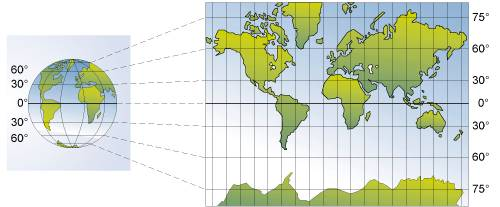
\includegraphics[width=#1]{images/mercator.jpg}
    \captionsetup{font={scriptsize}}
    \caption{#2}
  \end{figure}
}

\lstset{style=modernstyle}

\usetheme{Copenhagen}
\usecolortheme{default}
\setbeamertemplate{navigation symbols}{}

\title[exMA WP1 Vegetation]{
  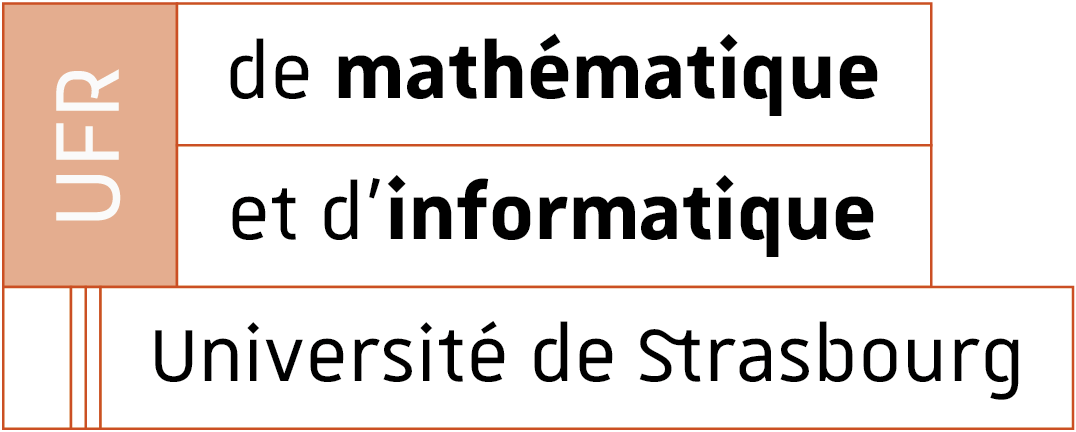
\includegraphics[width=0.8\textwidth]{images/logo_ufr.png}
  ExaMA WP1 - Vegetation}
\author[Carpi Lapi - Senger]{Giulio CARPI LAPI, Pierre-Antoine SENGER}

\begin{document}

\begin{frame}{Introduction}
  \titlepage
\end{frame}

\begin{frame}{Introduction}
  \Large
  \begin{itemize}
    \Large
    \item Part of the \textbf{HiDALGO2} project
    \item Specifically \textbf{Urban Building Model} use case
    \item Project conducted within \textbf{Cemosis} - \textbf{IRMA}
    \item Supervised by \textbf{Pierre Alliez} and \textbf{Vicent Chabannes}
  \end{itemize}
  \vfill % This adds vertical space to push the images to the bottom
  \centering
  \begin{minipage}{0.3\textwidth}
      \centering
      \includegraphics[width=0.8\textwidth]{images/hidalgo2.png}
  \end{minipage}
  \begin{minipage}{0.3\textwidth}
      \centering
      \includegraphics[width=0.8\textwidth]{images/logo-cemosis.png}
  \end{minipage}
  \begin{minipage}{0.3\textwidth}
      \centering
      \includegraphics[width=0.8\textwidth]{images/logo_irma.png}
  \end{minipage}
\end{frame}

\begin{frame}{Context}
  \Large
  \begin{figure}
      \centering
      \includegraphics[width=0.8\textwidth]{images/TreeShade.png}
      \captionsetup{font={scriptsize}}
      \caption{Tree providing shade to a building\cite{img:TreeShade}}
  \end{figure}
\end{frame}

\begin{frame}{Context}
  \Large
  \begin{figure}
      \centering
      \includegraphics[width=\textwidth]{images/heat_street.png}
      \captionsetup{font={scriptsize}}
      \caption{Thermal image of a street depicting heat distribution\cite{img:street_thermography}}
  \end{figure}
\end{frame}

\begin{frame}{Context}
  \Large
  \textbf{Main Goals:}
  \begin{itemize}
    \item Integrate \textbf{trees} into \textbf{3D geometric models} of \textbf{urban environments}
    \item Improve the \textbf{accuracy} of \textbf{thermal} and \textbf{energy simulations}
  \end{itemize}
\end{frame}


\begin{frame}{Context}
  \Large
\begin{figure}[H]
  \centering
  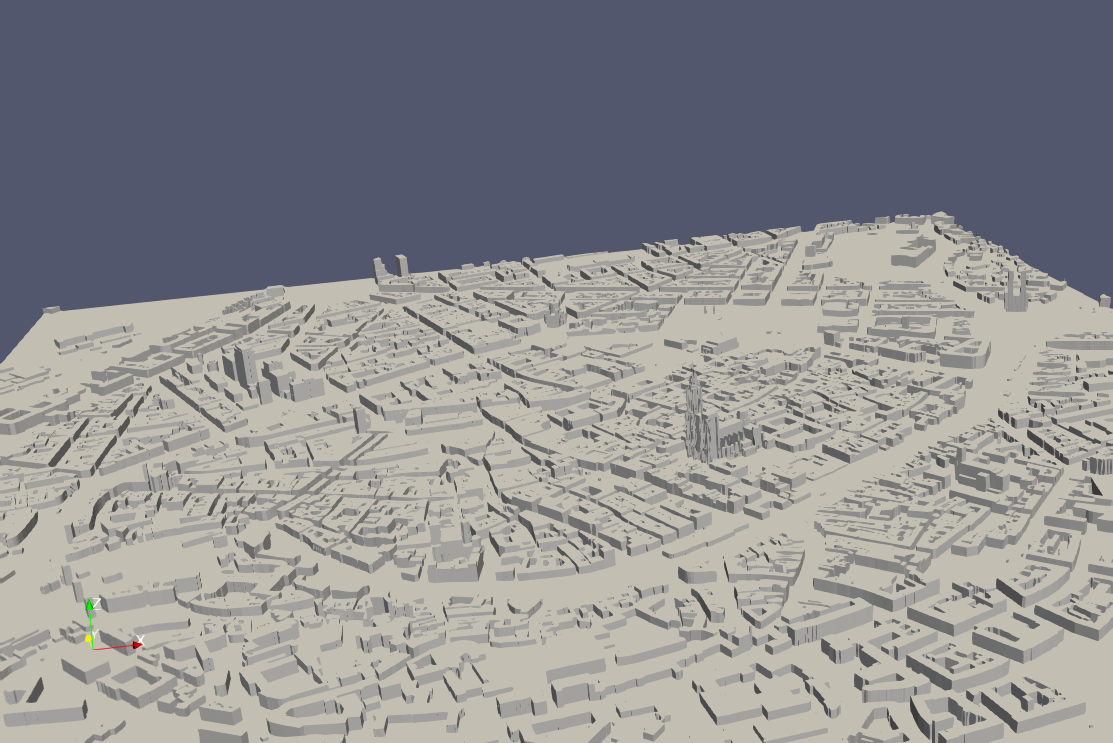
\includegraphics[width=0.8\textwidth]{images/stras_mesh.png}
  \captionsetup{font={scriptsize}}
  \caption{Strasbourg 3D model}
\end{figure}
\end{frame}

\begin{frame}{Context}
  \Large
\begin{figure}[H]
  \centering
  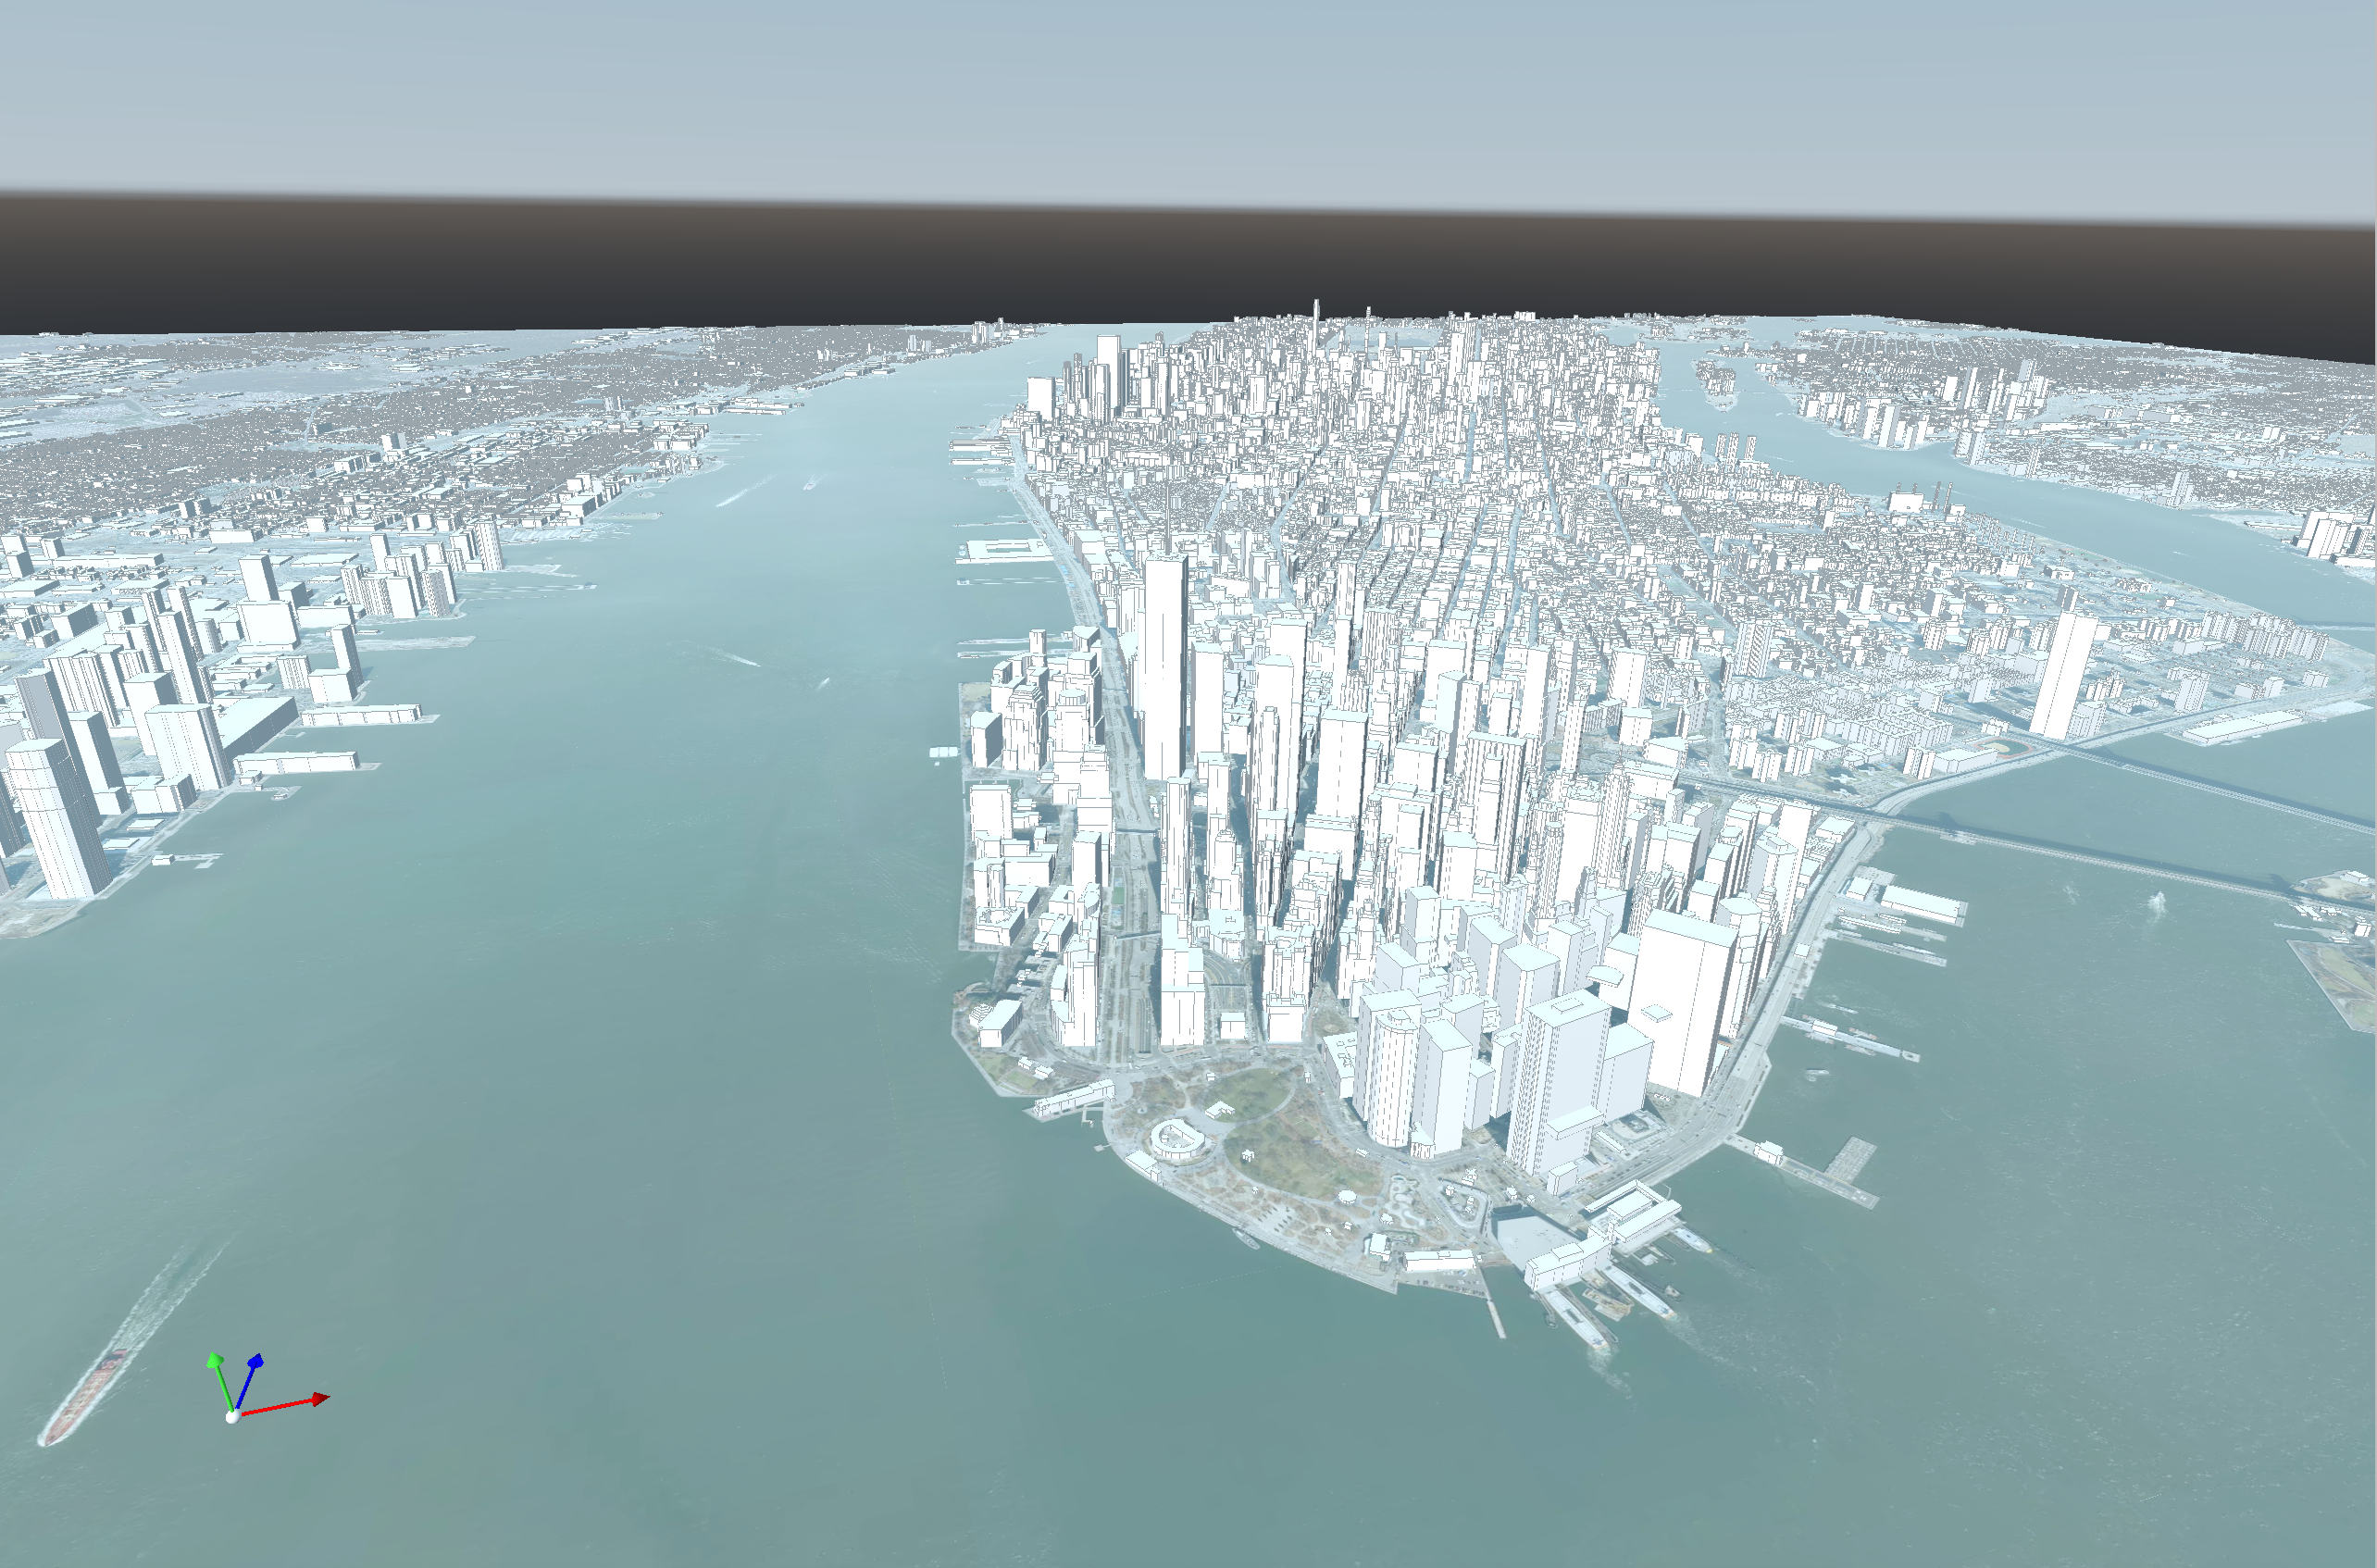
\includegraphics[width=0.8\textwidth]{images/manhattan_mesh.png}
  \captionsetup{font={scriptsize}}
  \caption{Manhattan 3D model}
\end{figure}
\end{frame}

\begin{frame}{Objectives}
  \Large
  \begin{itemize}
      \item \textbf{\textcolor{red}{Extracting}} \textbf{tree data} from \textbf{OpenStreetMap}
      \item \textbf{\textcolor{red}{Generating}} \textbf{3D tree models} using \textbf{CGAL}
      \item \textbf{\textcolor{red}{Integrating}} \textbf{tree models} in the \textbf{terrain mesh}
      \item \textbf{\textcolor{red}{Optimizing}} \textbf{computational efficiency}
      \item \textbf{\textcolor{red}{Delivering}} versions \textbf{V0}, \textbf{V1}, and \textbf{V2}
  \end{itemize}
\end{frame}

\begin{frame}{Sofware and libraries: Overpass API}
  \Large
  \begin{figure}[H]
      \centering
      \includegraphics[width=\textwidth]{images/OvAPI_logo.png}
  \end{figure}
  \begin{center}
  \Large \textbf{Overpass API} is a read-only API to query data from \textbf{OpenStreetMap}
  \end{center}
\end{frame}

\begin{frame}{Sofware and libraries: OpenStreetMap}
  \Large
  \begin{figure}[H]
      \centering
      
\includegraphics[width=0.5\textwidth]{images/osm_logo.png}
  \end{figure}
  \begin{center}
    \Large Collaborative free \textbf{geographic database}
  \end{center}
\end{frame}

\begin{frame}{Sofware and libraries: Overpass turbo}
  Overpass turbo is a web-based data filtering tool for OpenStreetMap. 
  It runs queries on the Overpass API.
  
    \begin{figure}[H]
      \centering
      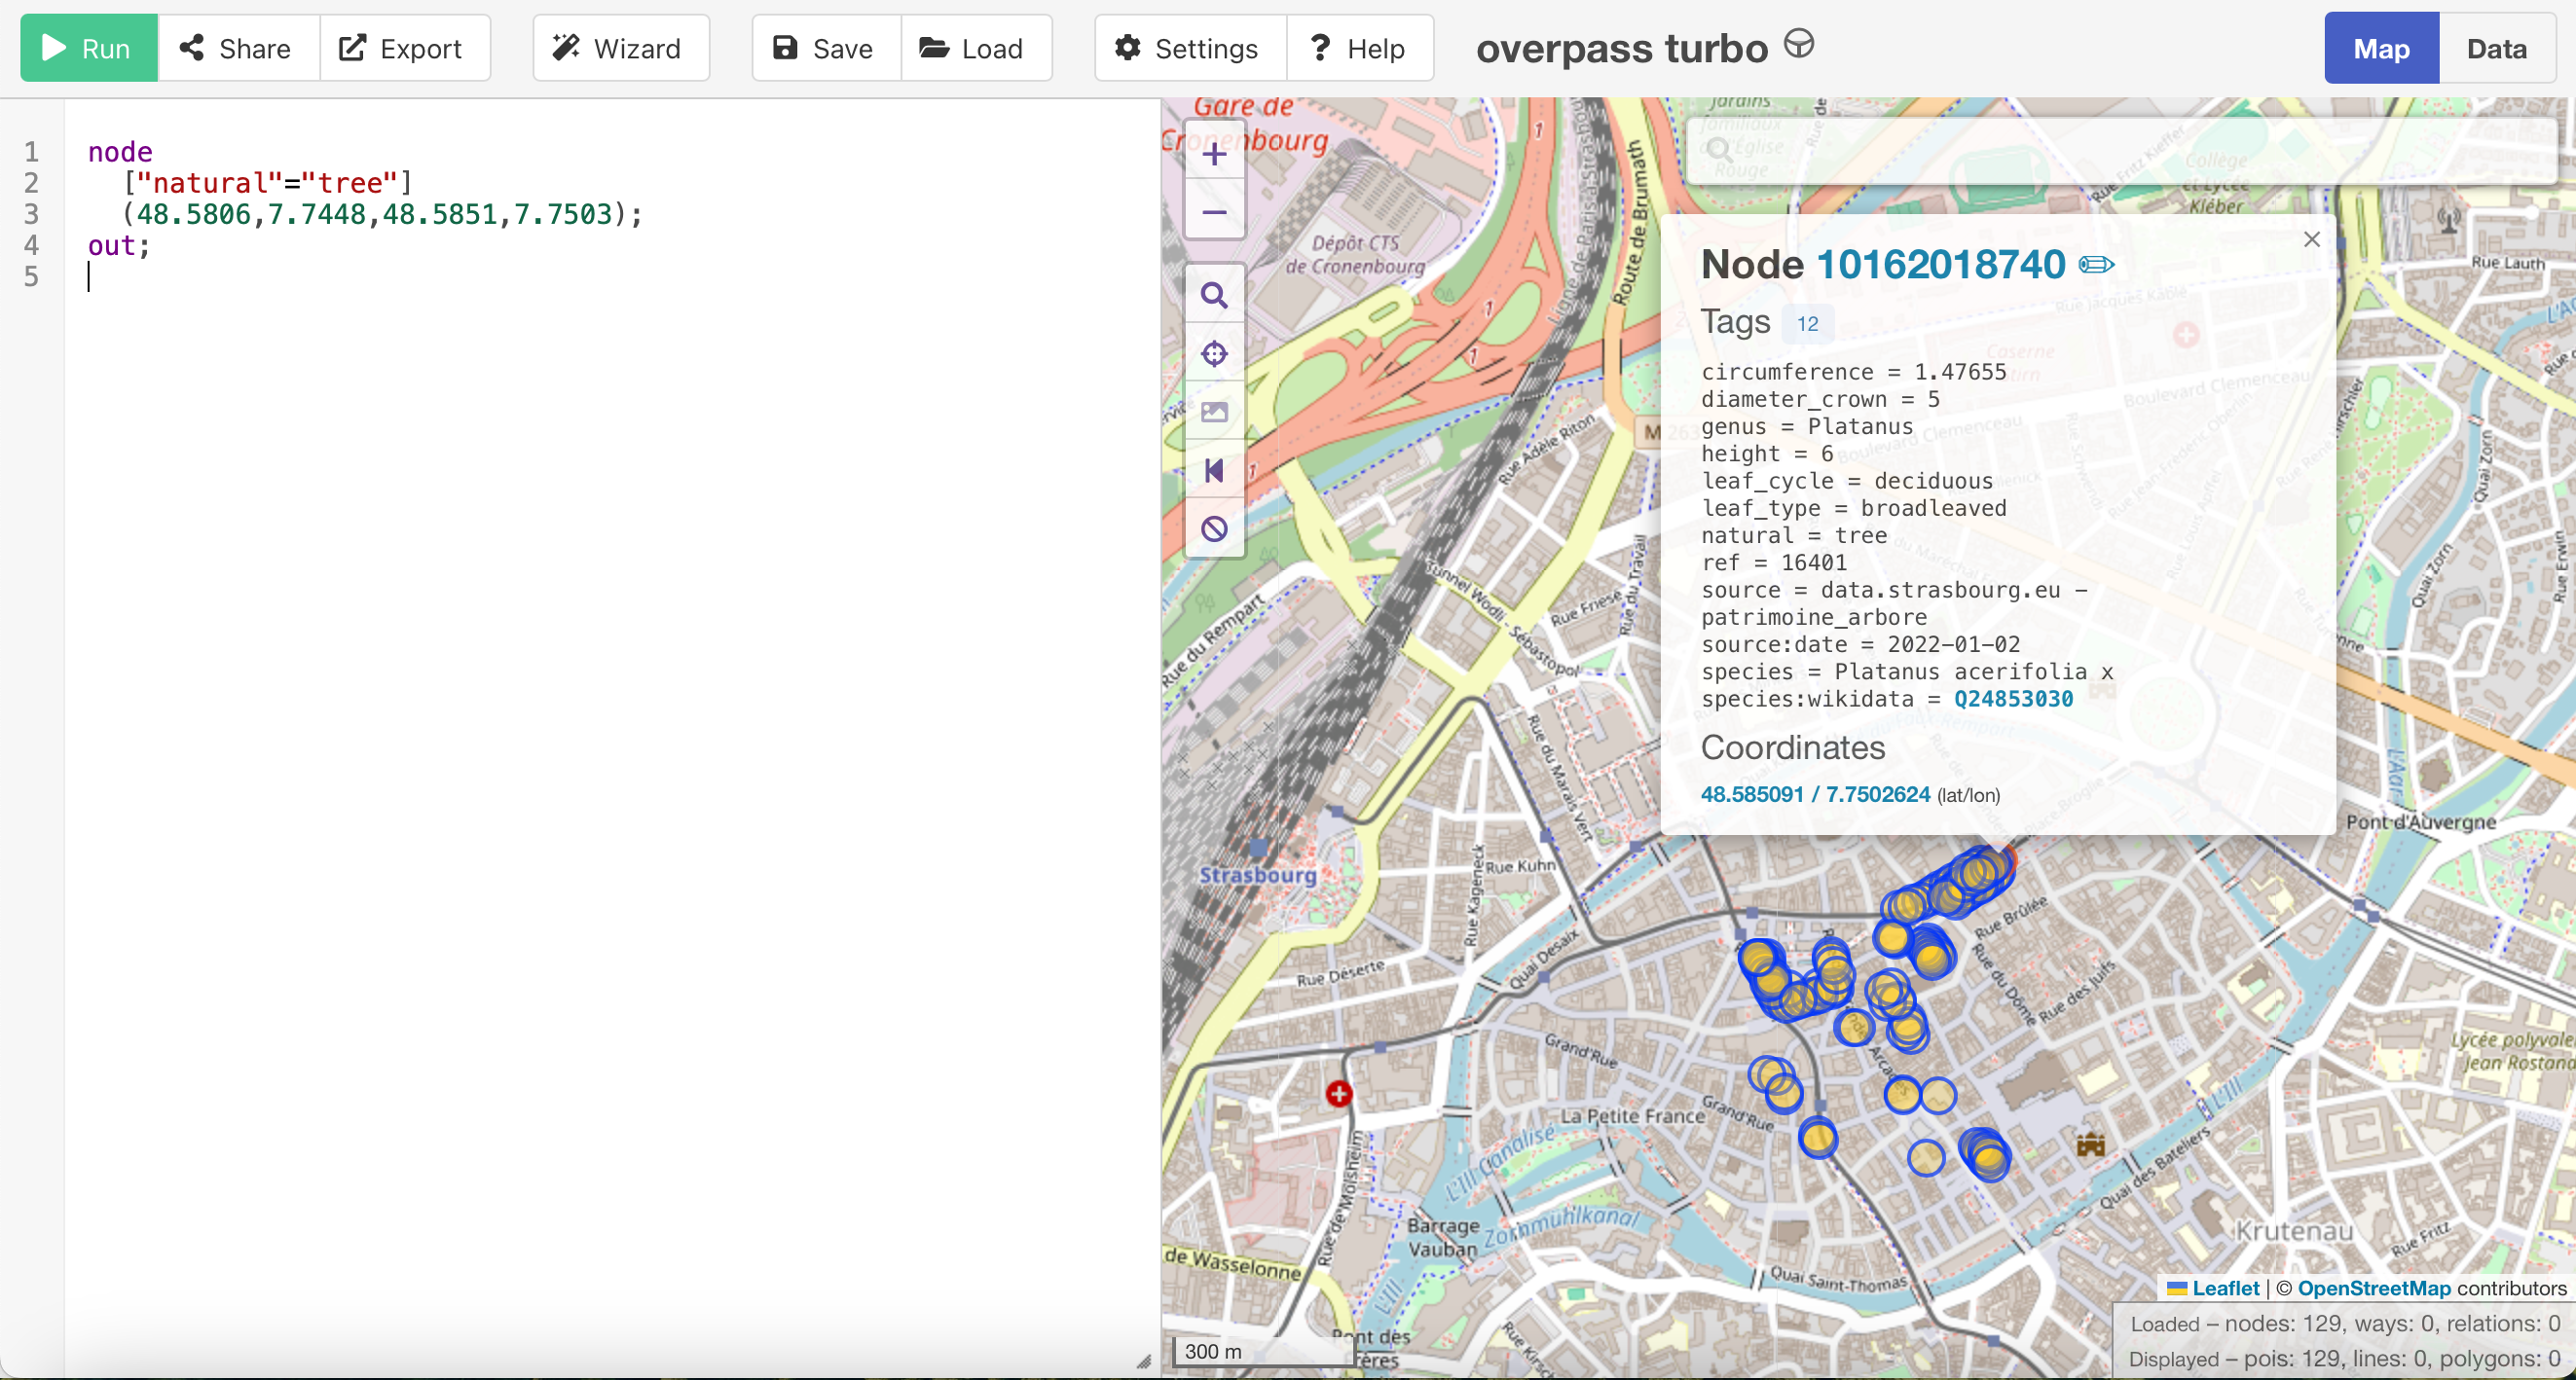
\includegraphics[width=\textwidth]{images/overpass-turbo.png}
      \captionsetup{font={scriptsize}}
      \caption{Query in Overpass turbo interface}
    \end{figure}
\end{frame}

\begin{frame}{Sofware and libraries: Overpass Turbo}
  \begin{figure}[H]
    \centering
    \includegraphics[width=0.75\textwidth]{images/ovt-node.png}
  \end{figure}
\end{frame}

\begin{frame}{Sofware and libraries: cURL}
  \Large
  \begin{figure}[H]
      \centering
      
\includegraphics[width=0.8\textwidth]{images/Curl-logo.svg.png}
  \end{figure}
  \begin{center}
    \Large \textbf{URL} transfer library
  \end{center}
\end{frame}

\begin{frame}{Sofware and libraries: how an API works}
  \begin{figure}[H]
    \centering
    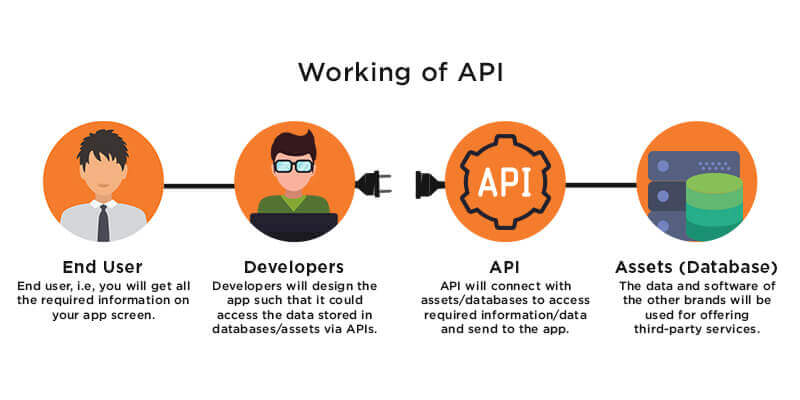
\includegraphics[width=1\textwidth]{images/how-api-works.jpg}
    \captionsetup{font={scriptsize}}
    \caption{Example of query to get trees in Strasbourg.}
  \end{figure}
\end{frame}

\begin{frame}{Sofware and libraries: CGAL}
  \Large
  \begin{figure}[H]
      \centering
      \includegraphics[width=0.8\textwidth]{images/cgal_logo.png}
  \end{figure}
  \begin{center}
    \Large Open source software library for \textbf{computational geometry algorithms}
  \end{center}
\end{frame}

\begin{frame}[fragile]{Methodology: Data acquisition}
  \textbf{Overpass API} and \textbf{cURL} to query
  \textbf{OpenStreetMap}
  \begin{lstlisting}[language=json]
curl_easy_setopt(curl, CURLOPT_URL,
                "http://overpass-api.de/api/interpreter");

// Set the Overpass query with the bounding box
std::string query =
"[out:json]; (node(" + bbox + ")[\"natural\"=\"tree\"];); out;";

std::cout << "Query: " << query << std::endl;
  \end{lstlisting}
\end{frame}


\begin{frame}[fragile]{Methodology: Data acquisition}
The data will be stored in a \textbf{.json} file:

\begin{lstlisting}[language=json]
{
    "type": "node",
    "id": 10161978695,
    "lat": 48.5872478,
    "lon": 7.7548520,
    "tags": {
        "circumference": "78.54",
        "diameter_crown": "5",
        "genus": "Tilia",
        "height": "10",
        "natural": "tree",
        "ref": "27466",
        "source": "data.strasbourg.eu - patrimoine_arbore",
        "source:date": "2022-01-02",
        "species": "Tilia euchlora x"
    }
}
\end{lstlisting}
\end{frame}

\begin{frame}[fragile]{Methodology: Data acquisition}
Sometimes, multiple \textbf{tags} are missing:

\begin{lstlisting}[language=json]
{
    "type": "node",
    "id": 4439566691,
    "lat": 48.5839128,
    "lon": 7.7487125,
    "tags": {
      "natural": "tree"
    }
}
\end{lstlisting}
\end{frame}

\begin{frame}[fragile]{Methodology: Data acquisition}
  \textbf{config.json} to specify the query parameters:
  \begin{lstlisting}[language=json]
  {
    "bbox": "48.5750,7.7394,48.5919,7.7621",
    "origin": "48.583055227464364, 7.748664426560083",
    "altitude": 0,
    "LOD": 3,
    "default_height_range": "3, 6",
    "default_genus": "Platanus",
    "input_building_mesh": "mesh_lod1.stl",
    "output_name": "grande_ile"
  }
  \end{lstlisting}
\end{frame}

\begin{frame}[fragile]{Tree library}
  \Large
\begin{lstlisting}[language=json]
{
    "known_genus": ["Abies",
                    "Acer",
                    "Aesculus",
                        ... ],
    "cedrus_like": [ "Chaemacyparis",
                    "Cupressus",
                        ... ],
    "acer_like": ["Fadus",
                "Metasequoia",
                "Sequoiadendron",
                ... ],
    "liquidambar_like": ["Liriodendron",
                        "Pyrus",
                        "Alnus",
                        ... ],
    "quercus_like": ["Corylus",
                    "Carya",
                    "Fagus",
                    ... ]
}
\end{lstlisting}
\end{frame}

\begin{frame}{Base tree model}
  \Large
\textbf{13} tree models from \textbf{SketchUp}:

\begin{figure}[H]
    \centering
        \centering
        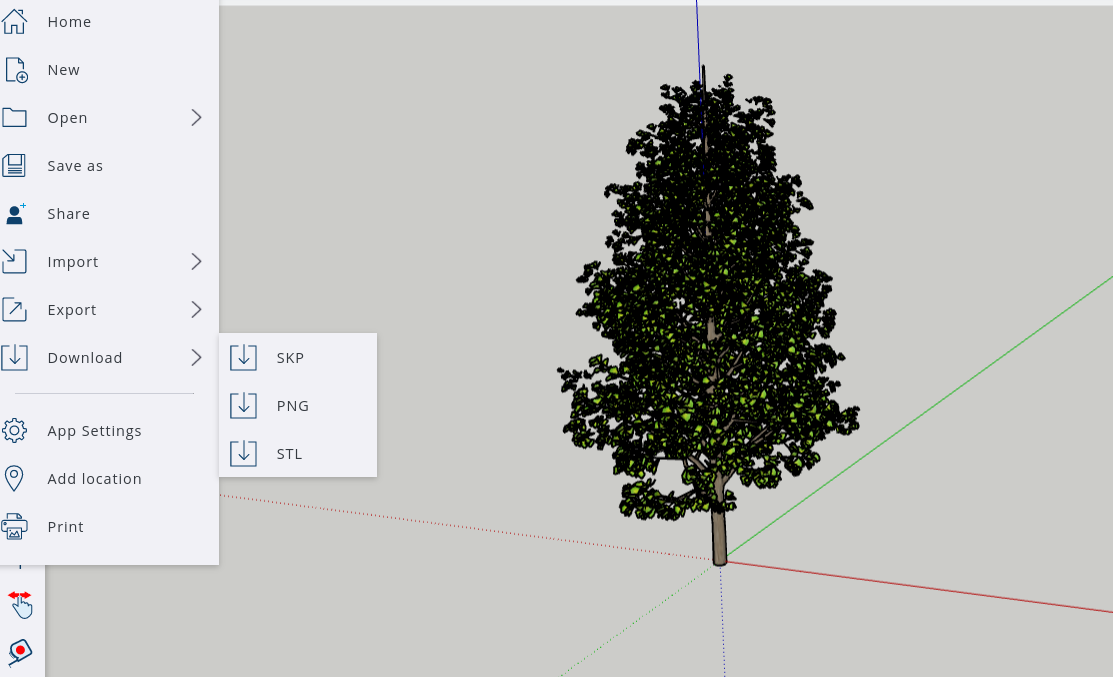
\includegraphics[width=0.8\textwidth]{images/ginkgo_sketchup.png}
        \captionsetup{font={scriptsize}}
        \caption{Mesh of a Ginkgo tree on Sketchup 3D Warehouse}
\end{figure}
\end{frame}

\begin{frame}{Base tree model}
  \Large
  \begin{figure}[H]
    \centering
    \begin{minipage}{0.24\textwidth}
        \centering
        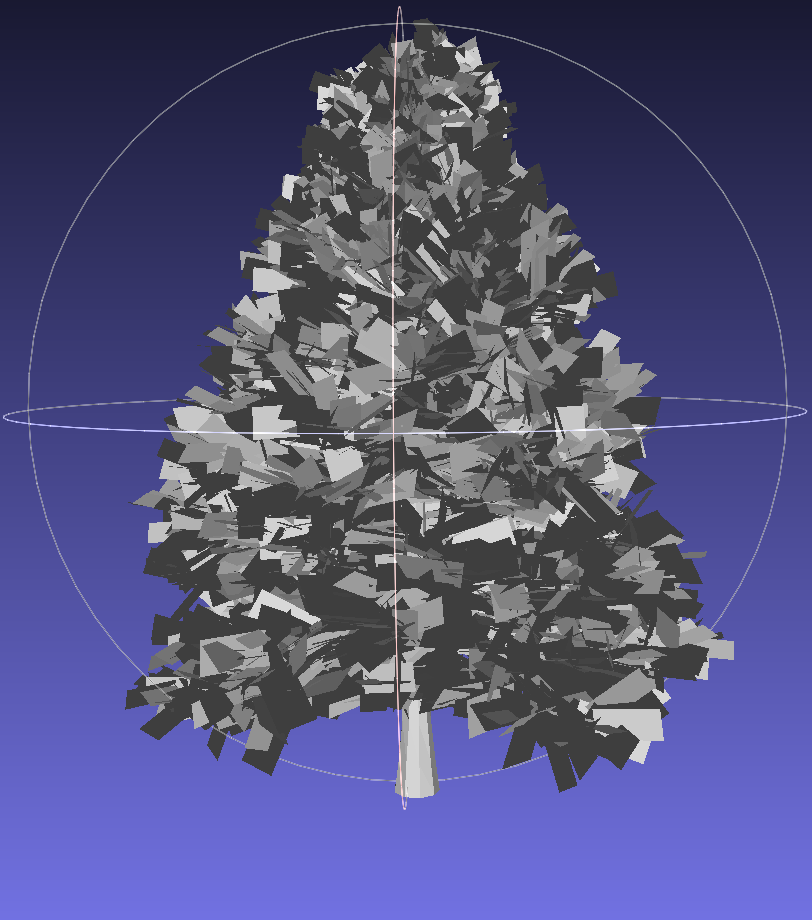
\includegraphics[width=\textwidth]{images/abies.png}
        \captionsetup{font={scriptsize}}
        \caption{Abies}
    \end{minipage}\hfill
    \begin{minipage}{0.24\textwidth}
        \centering
        \includegraphics[width=\textwidth]{images/acer.png}
        \captionsetup{font={scriptsize}}
        \caption{Acer}
    \end{minipage}\hfill
    \begin{minipage}{0.24\textwidth}
        \centering
        \includegraphics[width=\textwidth]{images/aesculus.png}
        \captionsetup{font={scriptsize}}
        \caption{Aesculus}
    \end{minipage}\hfill
    \begin{minipage}{0.24\textwidth}
        \centering
        \includegraphics[width=\textwidth]{images/catalpa.png}
        \captionsetup{font={scriptsize}}
        \caption{Catalpa}
    \end{minipage}
\end{figure}

\begin{figure}[H]
    \centering
    \begin{minipage}{0.24\textwidth}
        \centering
        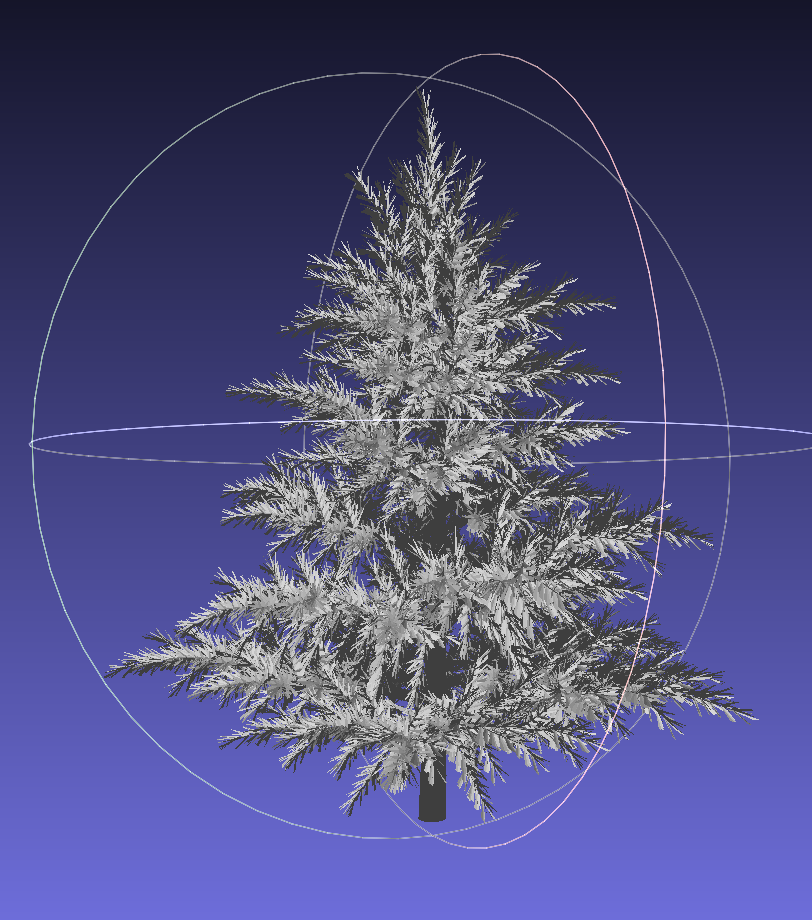
\includegraphics[width=\textwidth]{images/cedrus.png}
        \captionsetup{font={scriptsize}}
        \caption{Cedrus}
    \end{minipage}\hfill
    \begin{minipage}{0.24\textwidth}
        \centering
        \includegraphics[width=\textwidth]{images/liquidanbar.png}
        \captionsetup{font={scriptsize}}
        \caption{Liquidanbar}
    \end{minipage}\hfill
    \begin{minipage}{0.24\textwidth}
        \centering
        \includegraphics[width=\textwidth]{images/platanus.png}
        \captionsetup{font={scriptsize}}
        \caption{Platanus}
    \end{minipage}\hfill
    \begin{minipage}{0.24\textwidth}
        \centering
        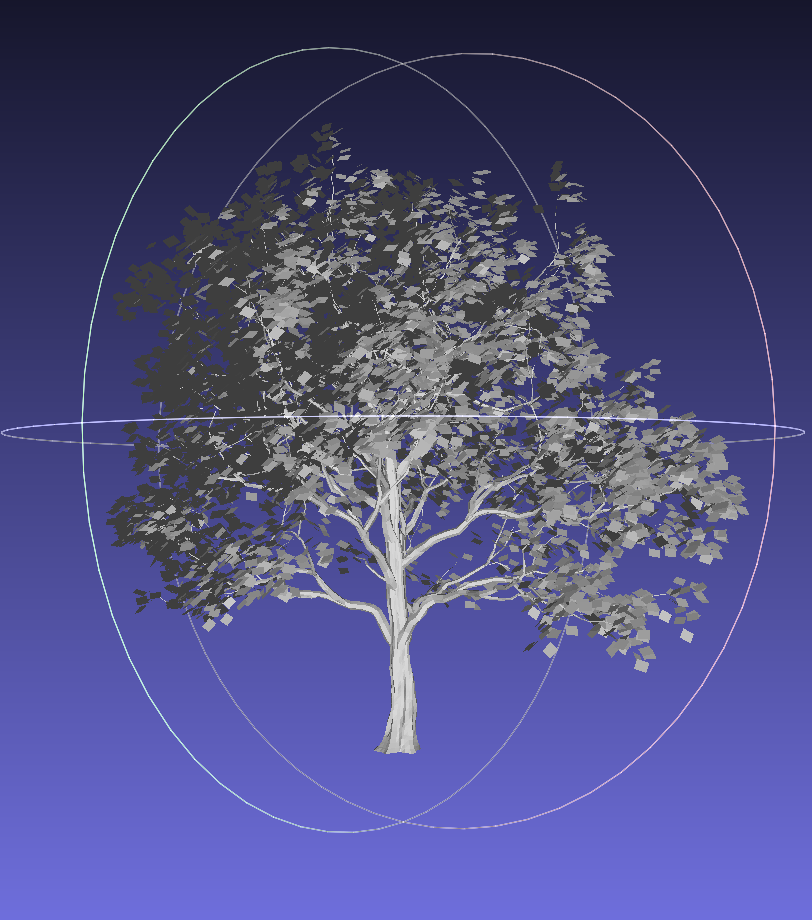
\includegraphics[width=\textwidth]{images/quercus.png}
        \captionsetup{font={scriptsize}}
        \caption{Quercus}
    \end{minipage}
\end{figure}
\end{frame}

\begin{frame}{Tree modeling: Alpha Wrapping}
  \Large
  To provide different LODs we will wrap then using the \texttt{CGAL 3D 
  Alpha Wrapping}
  \vfill
  \begin{figure}[H]
    \centering
        \centering
        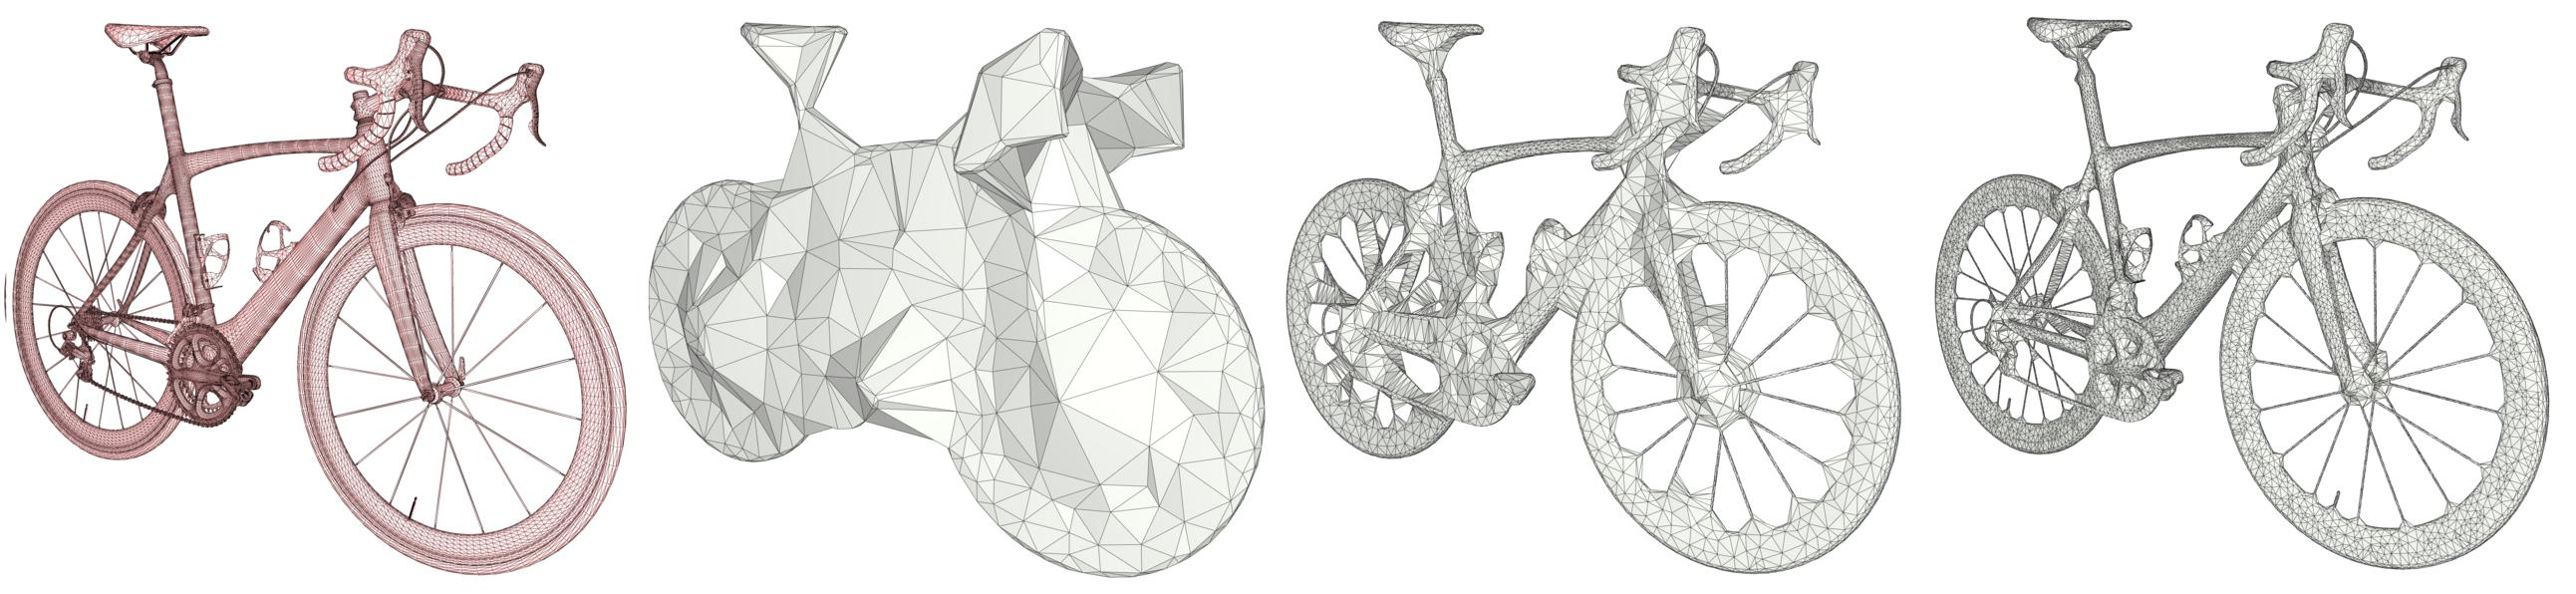
\includegraphics[width=\textwidth]{images/aw3_bike_lod.jpg}
        \captionsetup{font={scriptsize}}
        \caption{Different LOD of the Alpha Wrapping of a bike}
\end{figure}
\end{frame}

\begin{frame}{Reminder: Delaunay triangulation}
  \Large
  \begin{figure}[H]
    \centering
    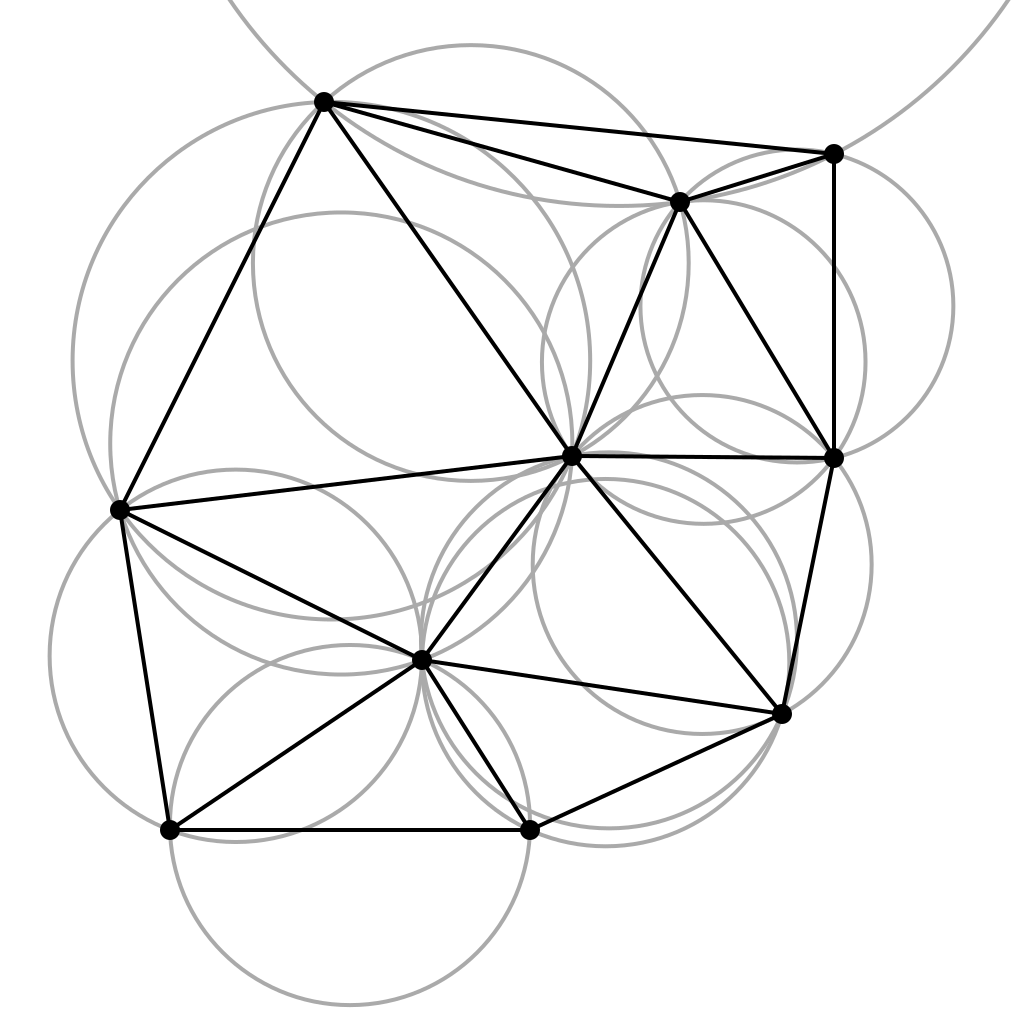
\includegraphics[width=0.6\textwidth]{images/Delaunay_circumcircles_vectorial.svg.png}
    \captionsetup{font={scriptsize}}
    \caption{Delaunay triangulation.
    The circumcircle of each triangle contains no other point}
\end{figure}
\end{frame}

\begin{frame}{Delaunay and Voronoi}
  \Large
  \begin{figure}[H]
    \centering
    \begin{minipage}{0.49\textwidth}
        \centering
        \includegraphics[width=\textwidth]{images/Delaunay_circumcircles_centers.svg.png}
        \captionsetup{font={scriptsize}}
        \caption{Delaunay triangulation with the centers of the circumcircles}
    \end{minipage}\hfill
    \begin{minipage}{0.49\textwidth}
        \centering
        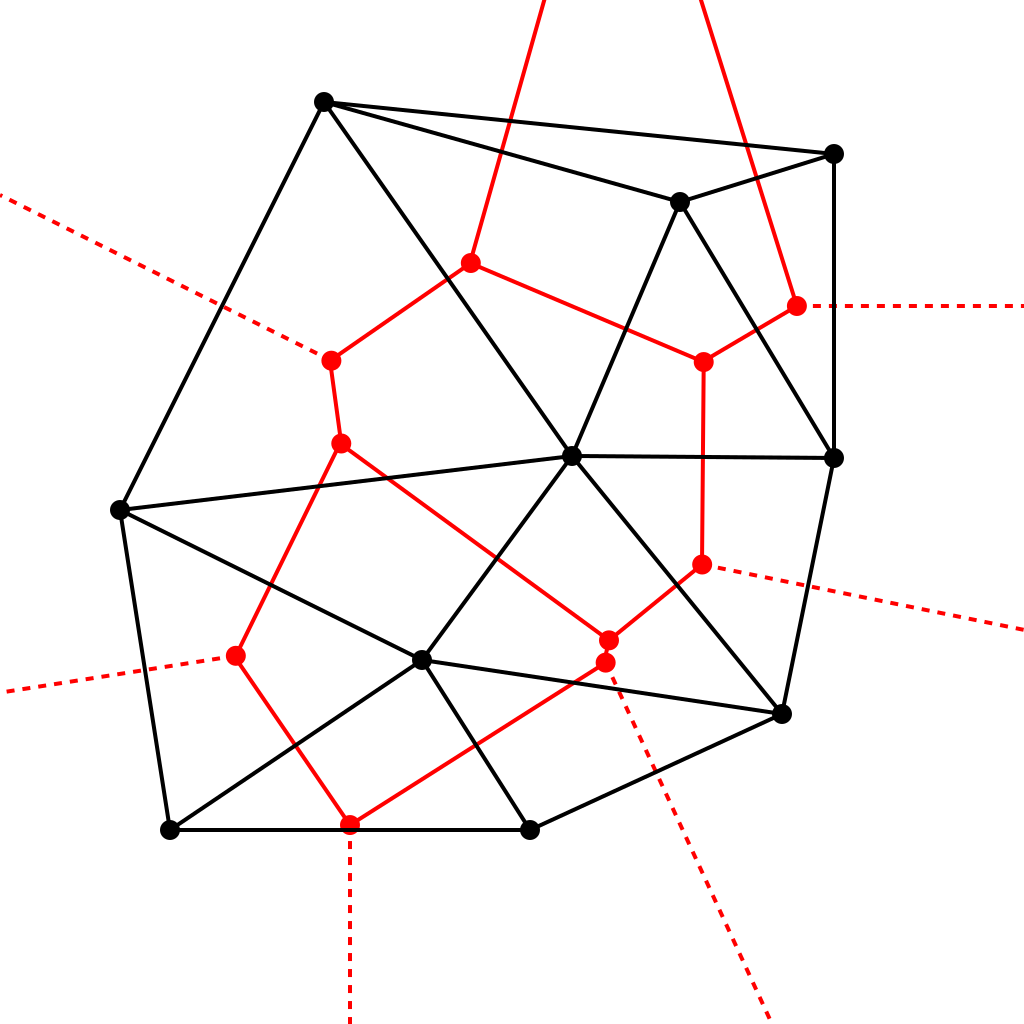
\includegraphics[width=\textwidth]{images/Delaunay_Voronoi.svg.png}
        \captionsetup{font={scriptsize}}
        \caption{The dual of the Delaunay triangulation, the Voronoi diagram}
    \end{minipage}
  \end{figure}
\end{frame}

\begin{frame}{Alpha Wrapping: Problem statement}
  \Large
  \textcolor{red}{\textbf{Input:}}
    \begin{itemize}
    \item  3D model with possible defects
    \end{itemize}
    \textcolor{red}{\textbf{Output:} }
    \begin{itemize}
      \item \textbf{Water-tight} mesh
      \item \textbf{No self-intersections}
      \item \textbf{Strictly enclosing the input}
      \item \textbf{Well shaped triangles}
    \end{itemize}
\end{frame}


\begin{frame}{Alpha Wrapping}
  \Large
  \begin{figure}[H]
    \centering
    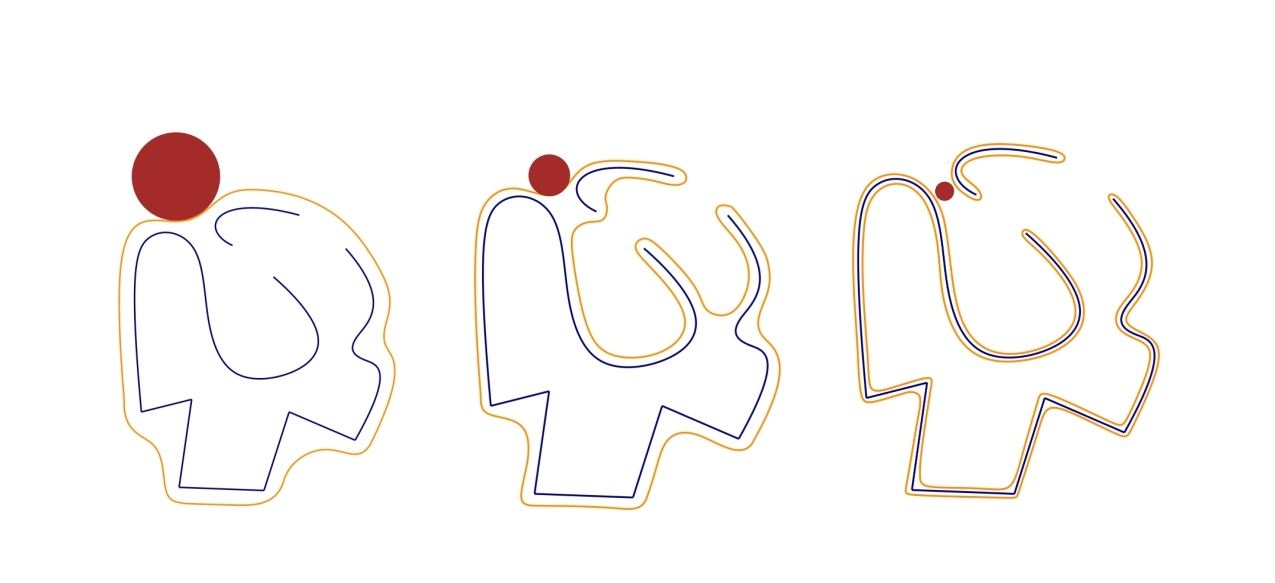
\includegraphics[width=1.1\textwidth]{images/alpha-wrapping_ball.jpg}
    \captionsetup{font={scriptsize}}
    \caption{Alpha Wrapping in 2D with Offset and different Alpha parameters}
\end{figure}
\end{frame}

\begin{frame}{Alpha Wrapping}
  \Large
  \begin{figure}[H]
    \centering
    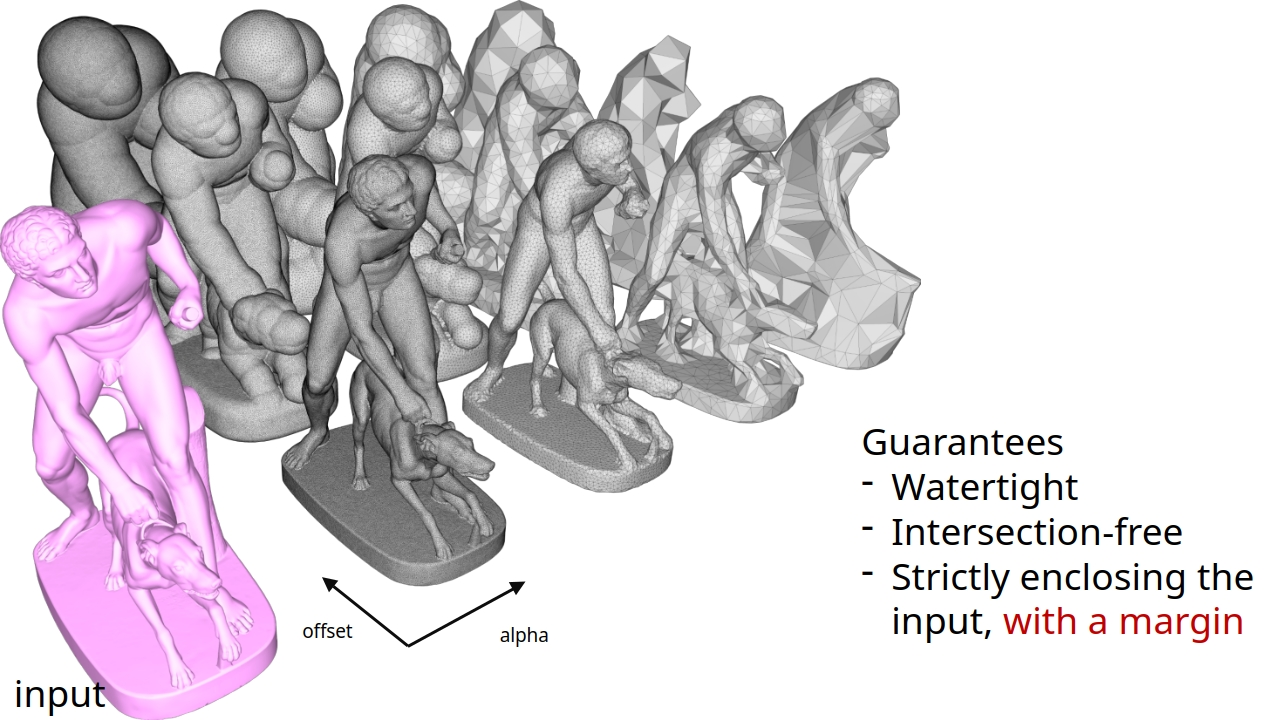
\includegraphics[width=1.1\textwidth]{images/alpha-wrapping_alpha_offset.jpg}
    \captionsetup{font={scriptsize}}
    \caption{Alpha Wrapping Alpha and Offset parameters}
\end{figure}
\end{frame}

\begin{frame}{Alpha Wrapping animation}
  \Large
  \href{https://youtu.be/xIIDolWCrgU}{video link}
  \begin{center}
    \movie[width=1\textwidth,height=0.8\textheight,poster,showcontrols]{}
    {images/alpha-wrapping-2d.mp4}
\end{center}
\end{frame}

\begin{frame}{Tree modeling: wrapping base tree}
  \Large
  \begin{figure}[H]
    \centering
    \begin{minipage}{0.49\textwidth}
        \centering
        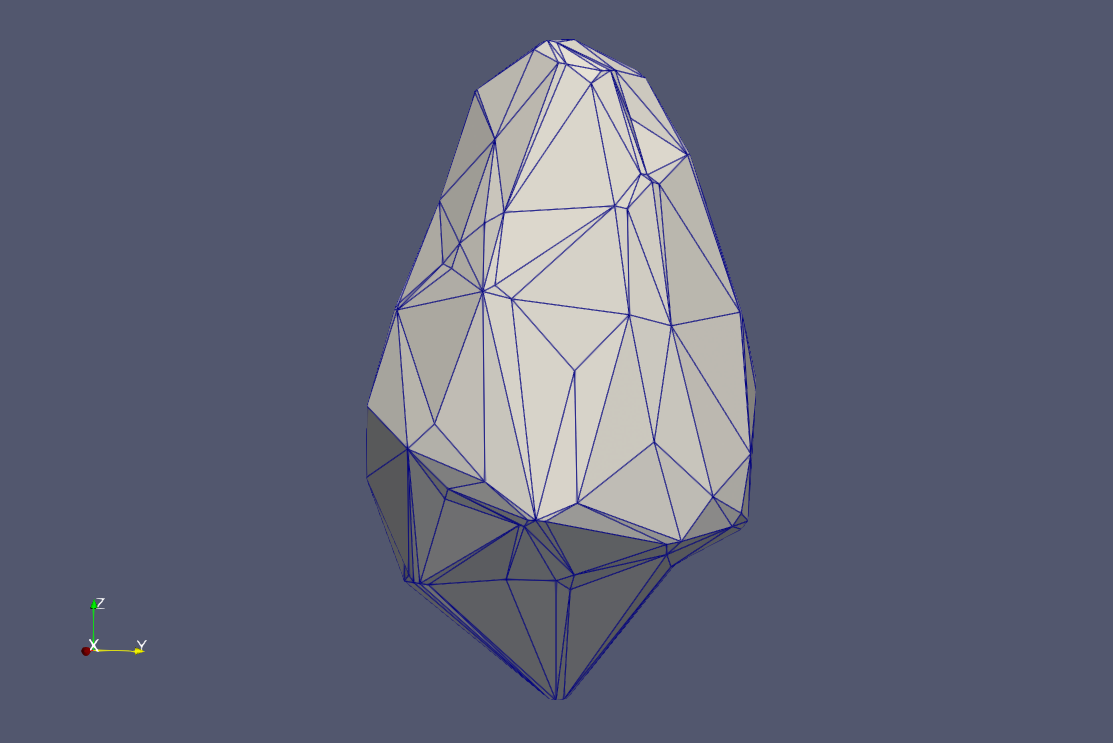
\includegraphics[width=0.8\textwidth]{images/gingko_lod0.png}
        \captionsetup{font={scriptsize}}
        \caption{Ginkgo lod0}
    \end{minipage}\hfill
    \begin{minipage}{0.49\textwidth}
        \centering
        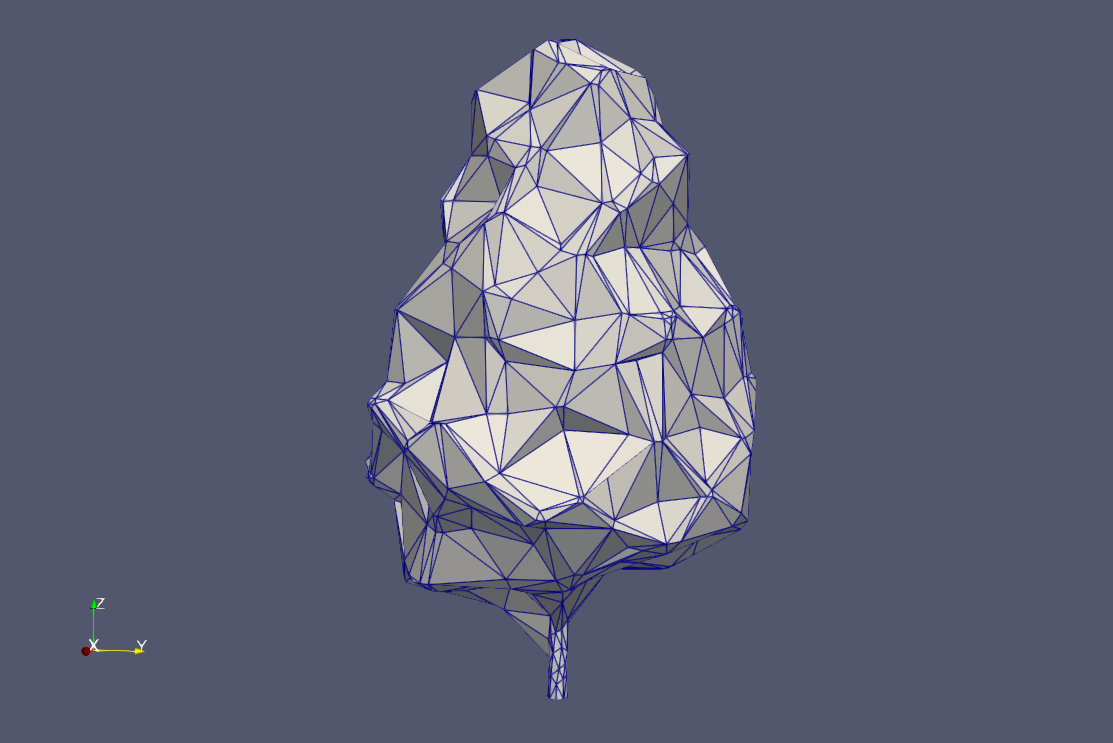
\includegraphics[width=0.8\textwidth]{images/gingko_lod1.png}
        \captionsetup{font={scriptsize}}
        \caption{Ginkgo lod1}
    \end{minipage}
\end{figure}

\begin{figure}[H]
    \centering
    \begin{minipage}{0.49\textwidth}
        \centering
        \includegraphics[width=0.8\textwidth]{images/gingko_lod2.png}
        \captionsetup{font={scriptsize}}
        \caption{Ginkgo lod2}
    \end{minipage}\hfill
    \begin{minipage}{0.49\textwidth}
        \centering
        \includegraphics[width=0.8\textwidth]{images/gingko_lod3.png}
        \captionsetup{font={scriptsize}}
        \caption{Ginkgo lod3}
    \end{minipage}
\end{figure}
\end{frame}

\begin{frame}{Mercator's projection}
  \Large
  \mercatorImage{Mercator's projection}

  \begin{itemize}
    \item \textbf{Most used} 
    \item \textbf{Conformal} 
    \item \textbf{Distortion} 
  \end{itemize}
\end{frame}

\begin{frame}{Mercator's projection}
  \Large
  \mercatorImage{Mercator's projection}
  A(latitude, longitude) = A($\phi$, $\lambda$),\\
  \begin{equation}
    \text{projection} \Longrightarrow \quad
    \left\{
    \begin{array}{l}
        x =  \lambda - \lambda_{0} \\
        y =  \ln(\tan(\frac{\pi}{4} + \frac{\phi}{2}))
    \end{array}
    \right.
  \end{equation}
  ,where $\lambda_{0}$ is the center of the map
\end{frame}

\begin{frame}{Mercator's projection}
  \Large
  \mercatorImage{Mercator's projection}
  But the Earth isn't a perfect sphere...
\end{frame}


\begin{frame}{Mercator's projection}
  \Large
  \begin{figure}[H]
    \centering
    \begin{minipage}{0.49\textwidth}
        \centering
        \includegraphics[width=0.8\textwidth]{images/WGS84_mean_Earth_radius.svg.png}
        \captionsetup{font={scriptsize}}
        \caption{Earth as an ellipsoid}
    \end{minipage}\hfill
    \begin{minipage}{0.49\textwidth}
        \centering
        
\includegraphics[width=0.8\textwidth]{images/WGS_84_reference_frame.png}
        \captionsetup{font={scriptsize}}
        \caption{WGS 84 reference frame}
    \end{minipage}
\end{figure}

\textit{WGS84toCartesian.hpp} $\Longrightarrow$ \textbf{GPS} to \textbf{Cartesian} coordinates.
\end{frame}

\begin{frame}{Modeling trees in 3D space}
  \Large
\texttt{CGAL Affine Transformation} \\
(complexity in $O(n)$)

\begin{figure}[H]
  \centering
  \begin{minipage}{0.49\textwidth}
      \centering
      \includegraphics[width=1\textwidth]{images/republic_lod3.png}
      \captionsetup{font={scriptsize}}
      \caption{Republic square with LOD 3 trees.}
  \end{minipage}\hfill
  \begin{minipage}{0.49\textwidth}
      \centering
      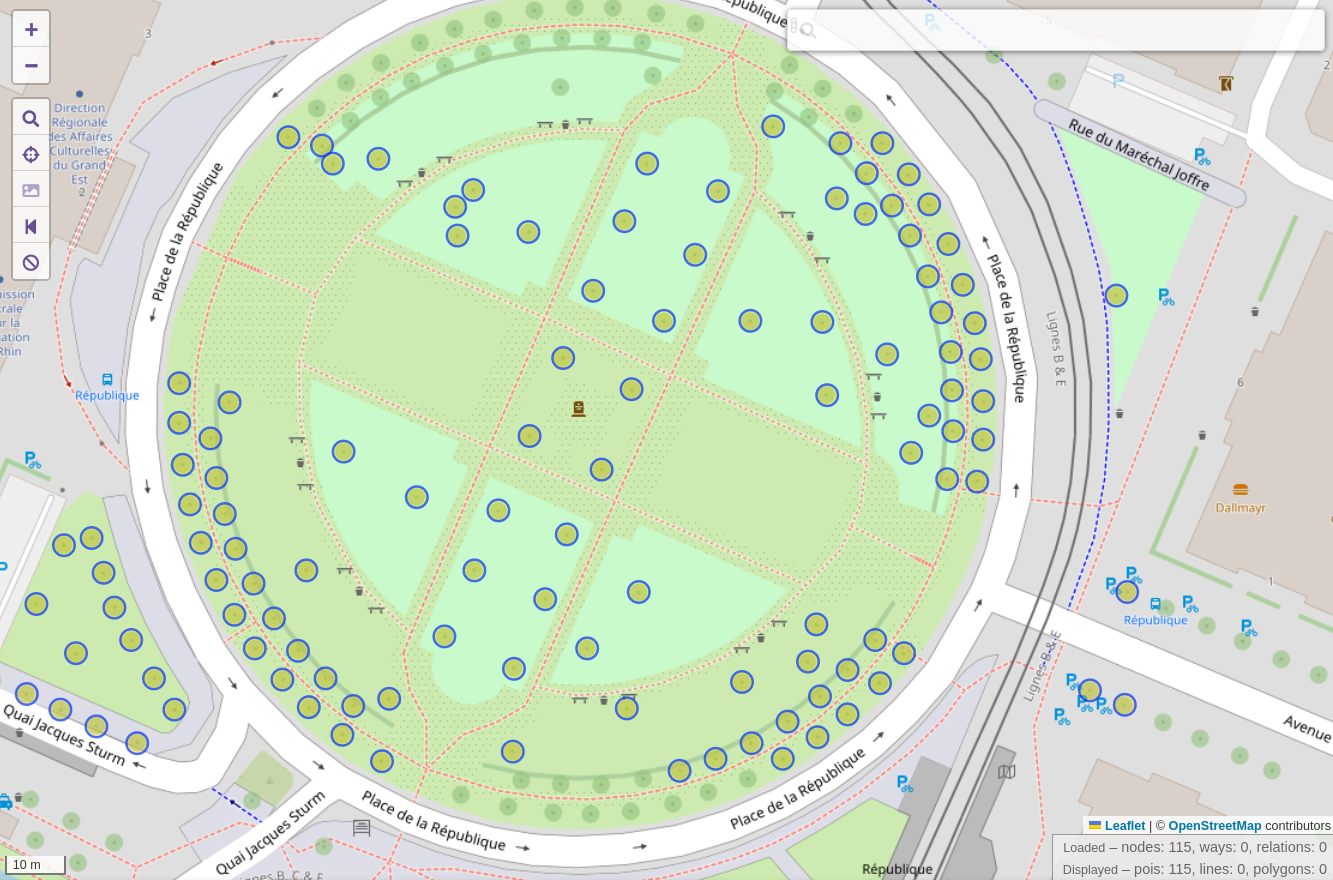
\includegraphics[width=1\textwidth]{images/republic_overpassturbo.png}
      \captionsetup{font={scriptsize}}
      \caption{Republic square trees from Overpass turbo}
  \end{minipage}
\end{figure}
\end{frame}

\begin{frame}{Modeling trees in 3D space}
  \Large
  \begin{figure}[H]
    \centering
    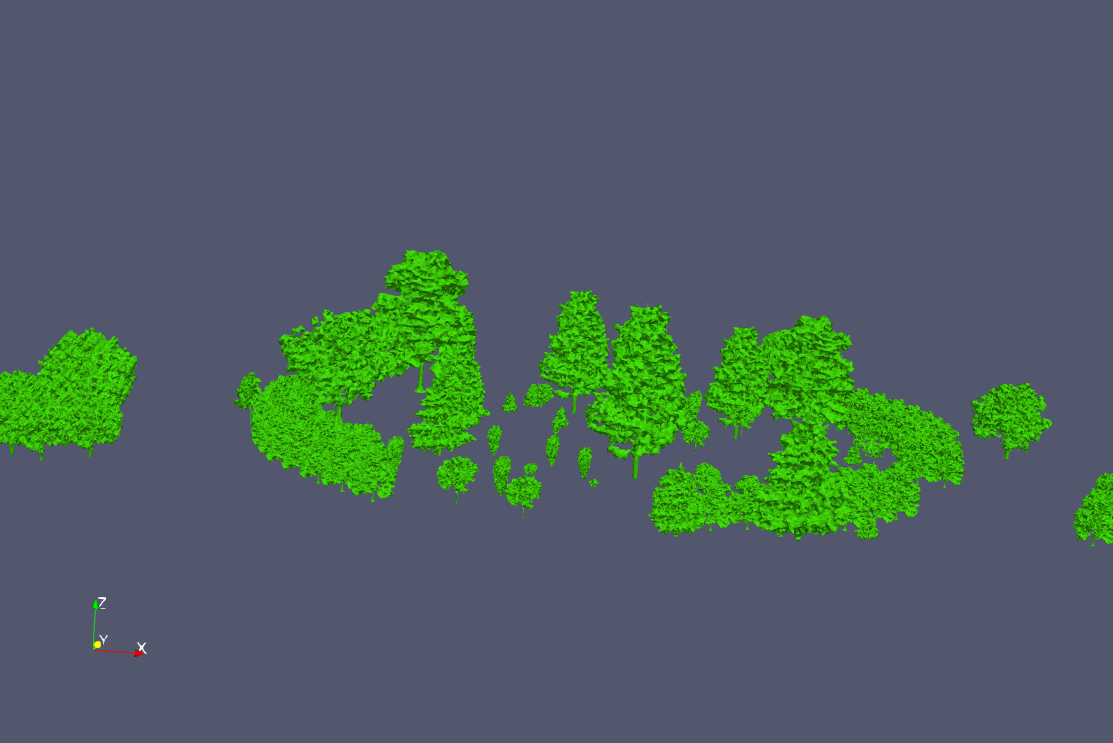
\includegraphics[width=1\textwidth]{images/republic_lod3_side.png}
    \captionsetup{font={scriptsize}}
    \caption{Side view of Republic square with LOD 3 trees}
\end{figure}
\end{frame}

\begin{frame}{Model integration}
  \Large
  \begin{figure}[H]
    \centering
    \includegraphics[width=1\textwidth]{images/strasbourg_mesh_enhanced1.png}
    \captionsetup{font={scriptsize}}
    \caption{Strasbourg 3D model with LOD 0 trees}
\end{figure}
\end{frame}

\begin{frame}{Model integration}
  \Large
  \begin{figure}[H]
    \centering
    \includegraphics[width=1\textwidth]{images/strasbourg_mesh_enhanced2.png}
    \captionsetup{font={scriptsize}}
    \caption{Strasbourg 3D model with LOD 0 trees}
\end{figure}
\end{frame}

\begin{frame}{Model integration: prospects}
  \Large
  Prospects: 
  \begin{itemize}
    \item \texttt{Feel++} $\Longrightarrow$ shading calculations
    \item Mesh$\Longrightarrow$ Hungarian team.
  \end{itemize}
  \href{https://youtu.be/O6flpW6jR60}{video link}
  \begin{center}
    \movie[width=1\textwidth,height=0.7\textheight,poster,showcontrols]{}{images/SolarMask.mp4}
\end{center}
\end{frame}

\begin{frame}{Benchmark: bbox 1}
  \Large
  \begin{figure}[H]
    \centering
    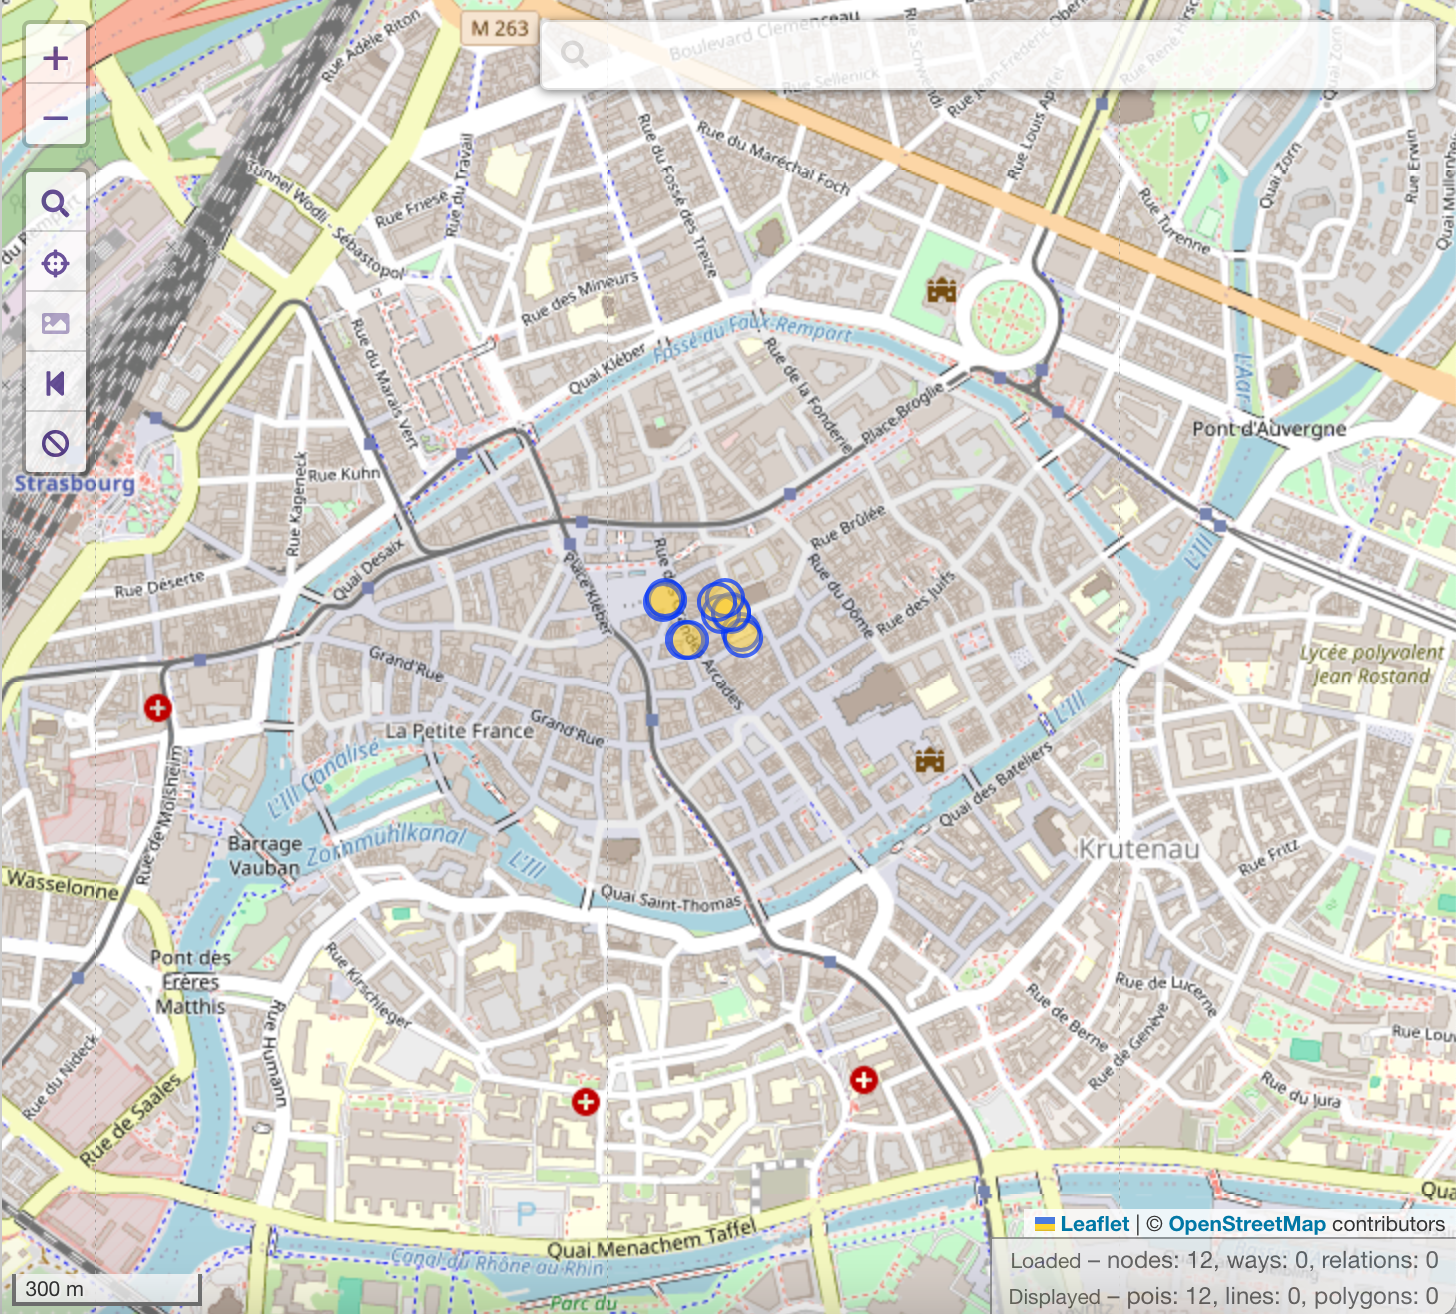
\includegraphics[width=0.7\textwidth]{images/bbox1.png}
    \captionsetup{font={scriptsize}}
    \caption{Bounding Box 1: 153.7 m², 12 trees}
\end{figure}
\end{frame}

\begin{frame}{Benchmark: bbox 2}
  \Large
  \begin{figure}[H]
    \centering
    \includegraphics[width=0.7\textwidth]{images/bbox2.png}
    \captionsetup{font={scriptsize}}
    \caption{Bounding Box 2: 384.0 m², 71 trees}
\end{figure}
\end{frame}

\begin{frame}{Benchmark: bbox 3}
  \Large
  \begin{figure}[H]
    \centering
    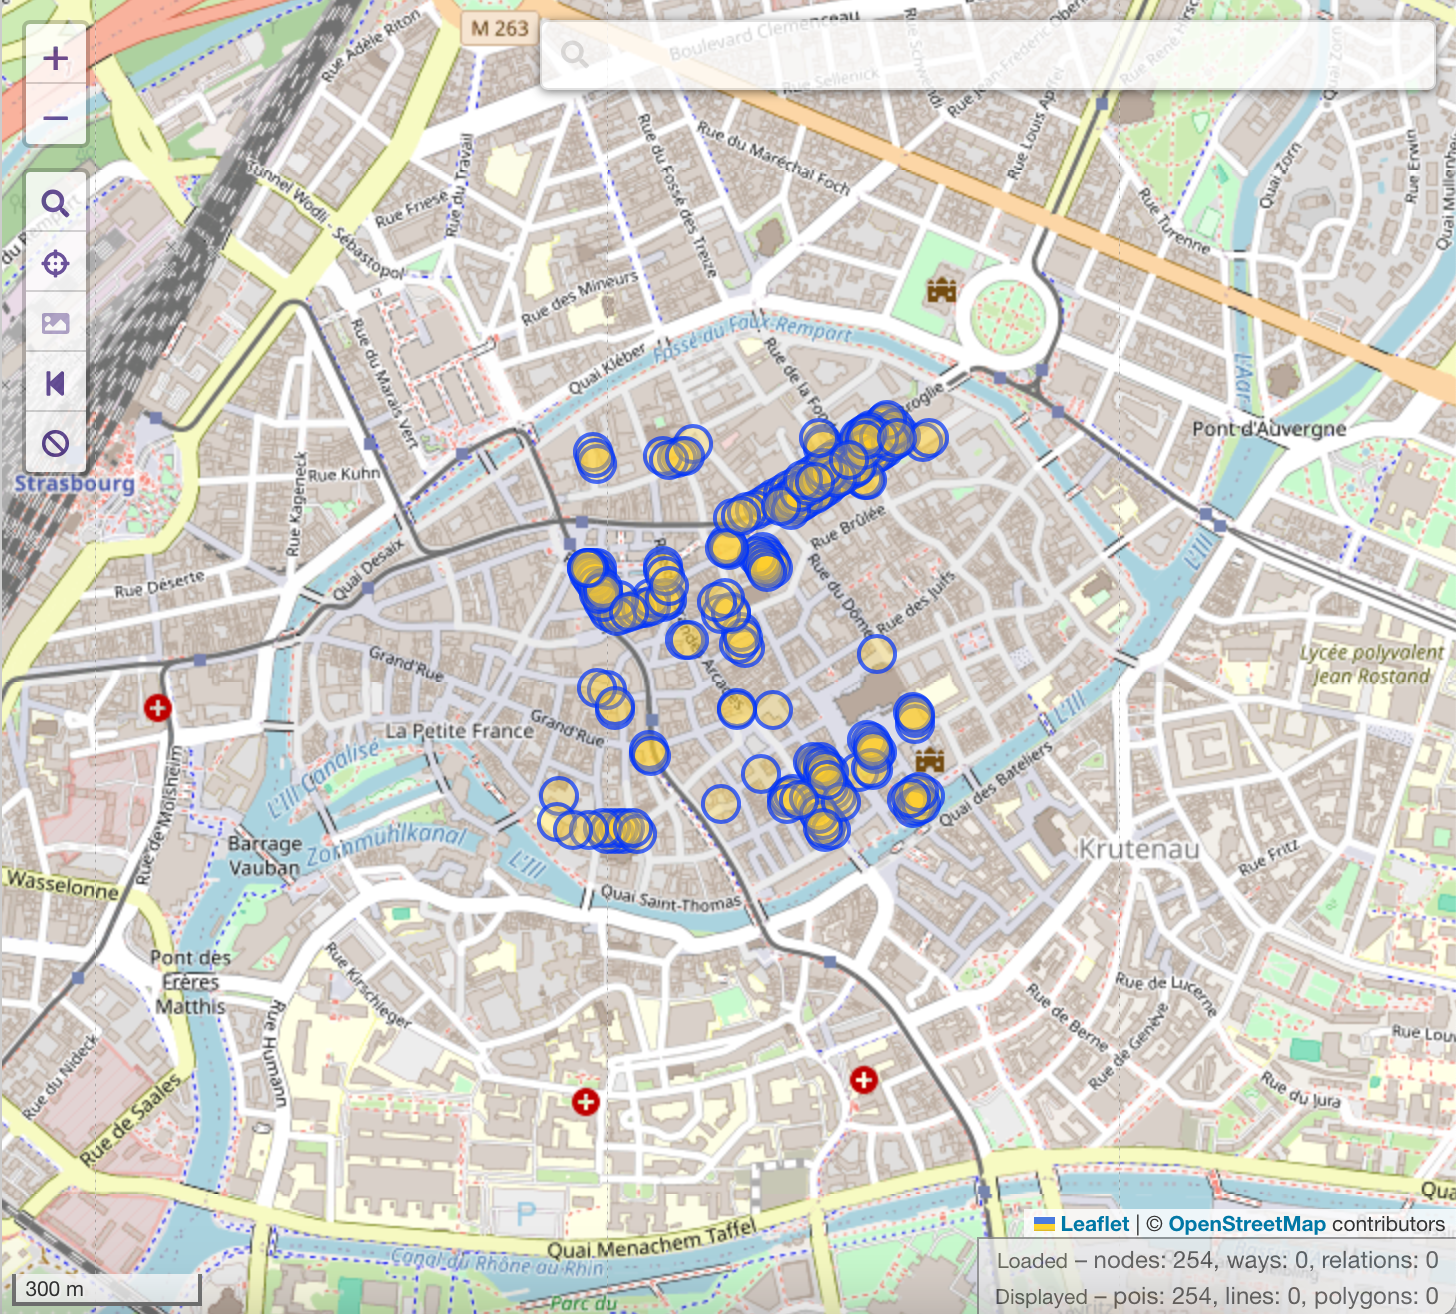
\includegraphics[width=0.7\textwidth]{images/bbox3.png}
    \captionsetup{font={scriptsize}}
    \caption{Bounding Box 3: 626.1 m², 254 trees}
\end{figure}
\end{frame}

\begin{frame}{Benchmark: bbox 4}
  \Large
  \begin{figure}[H]
    \centering
    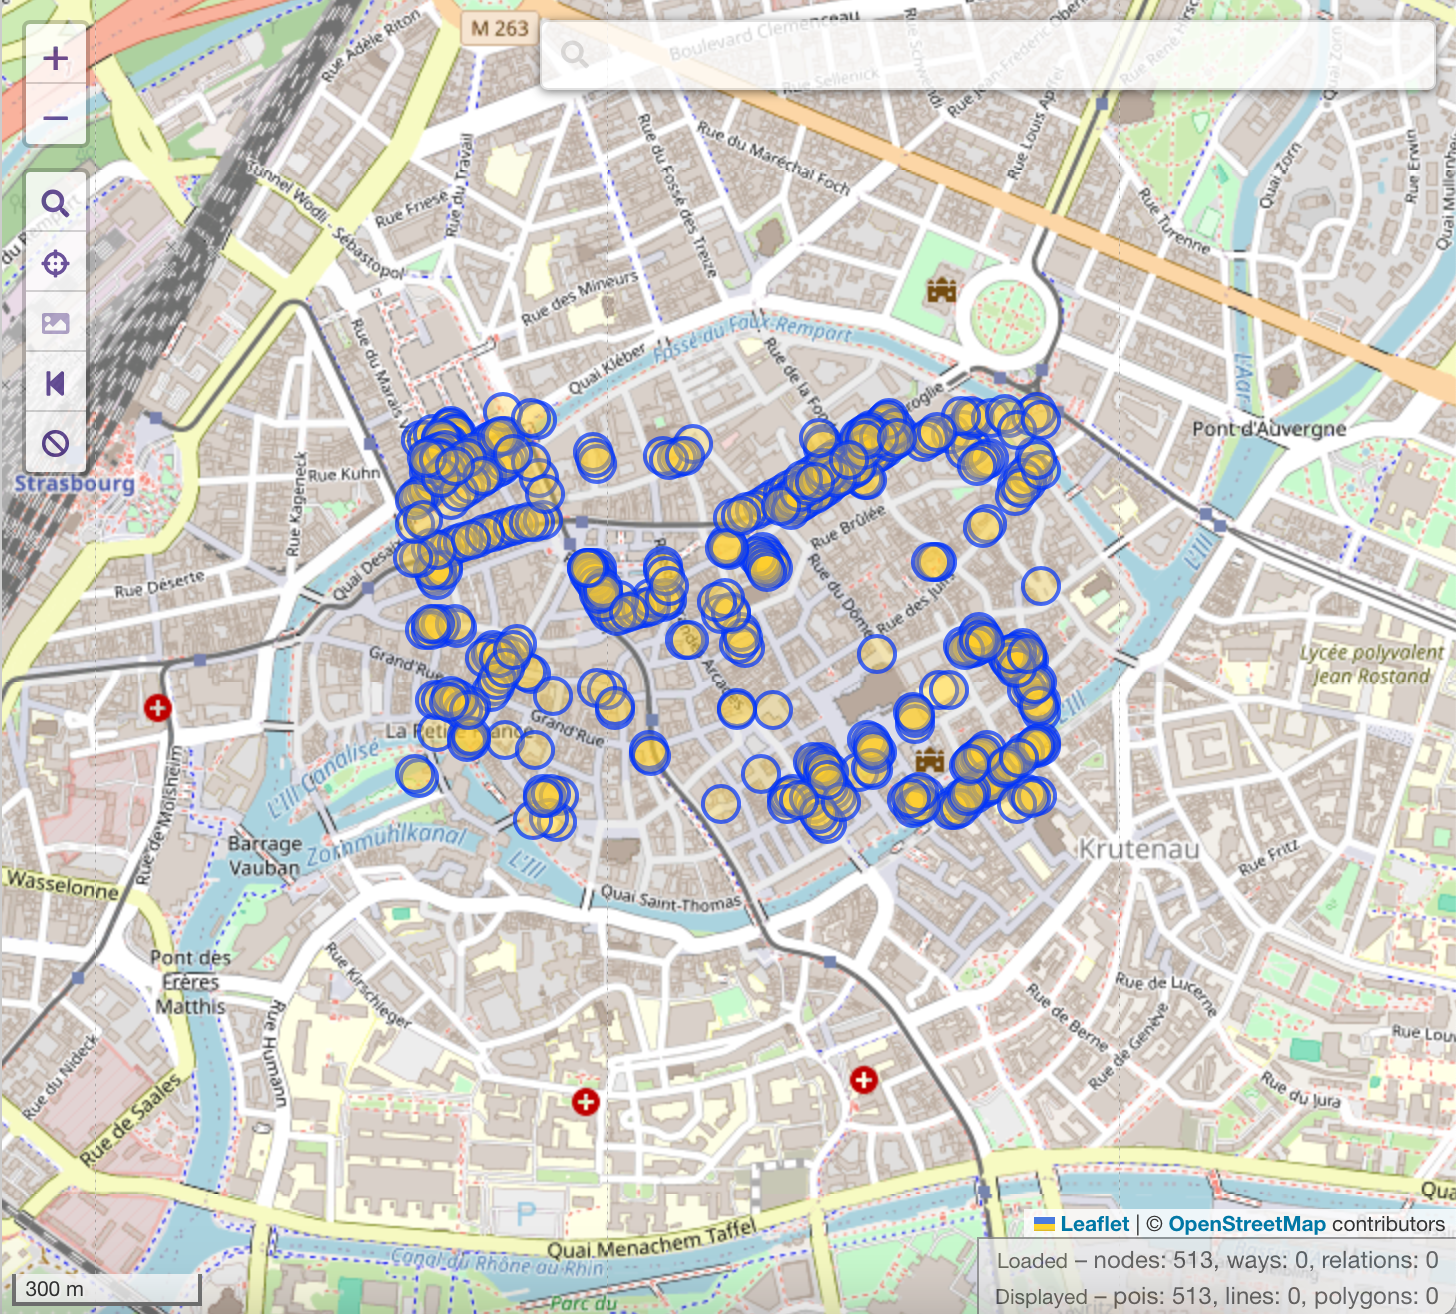
\includegraphics[width=0.7\textwidth]{images/bbox4.png}
    \captionsetup{font={scriptsize}}
    \caption{Bounding Box 4: 808.4 m², 513 trees}
\end{figure}
\end{frame}

\begin{frame}{Benchmark: relation LOD-number of faces}
  \Large
  \begin{figure}[H]
    \centering
    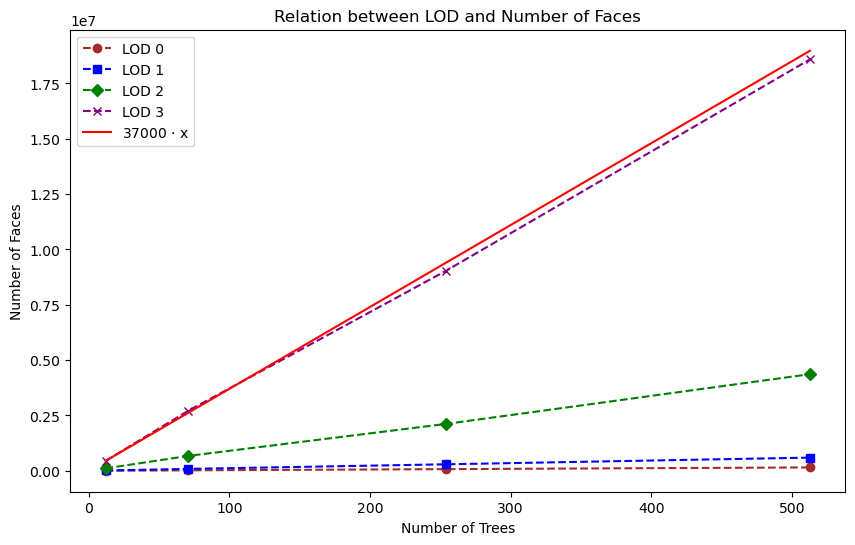
\includegraphics[width=1\textwidth]{images/bench_ntree_nfaces.png}
    \captionsetup{font={scriptsize}}
\end{figure}
\end{frame}

\begin{frame}{Benchmark: execution time (Part 1)}
  \Large
  \begin{figure}[H]
    \centering
    \includegraphics[width=1\textwidth]{images/bench_time_ntree_quad.png}
    \captionsetup{font={scriptsize}}
    \caption{\texttt{corefine\_and\_compute\_union}}
  \end{figure}
\end{frame}

\begin{frame}{Benchmark: execution time (Part 2)}
  \Large
  \begin{figure}[H]
    \centering
    \includegraphics[width=1\textwidth]{images/bench_time_ntree_linear.png}
    \captionsetup{font={scriptsize}}
    \caption{\texttt{autorefine\_triangle\_soup}}
  \end{figure}
\end{frame}


\nocite{*}
\bibliographystyle{unsrt}
\bibliography{references}

\end{document}